\chapter{OCL Constraint Interpretation}
\label{chapter:interpretation}

\begin{flushright}
\textit{Chapter written by Claas Wilke}
\end{flushright}

This Chapter describes how the \acs{OCL}2 Interpreter provided with \acl{DOT4Eclipse} can be used. How to install and run \keyword{Dresden OCL2 for Eclipse} and how to load models and OCL constraints will not be explained in this Chapter. This Chapter assumes that the user is familiar with such basic uses of the toolkit. A general introduction into \acl{DOT4Eclipse} can be found in Chapter \ref{chapter:introduction}.




\section{The Simple Example}

This Chapter uses the \keyword{Simple Example} which is provided with \acl{DOT4Eclipse} located in the plug-in package \reference{tudresden.ocl20.pivot.examples.\linebreak[0]simple}. An overview over all examples provided with \acl{DOT4Eclipse} can be found in \ref{tab:examples}. An introduction into the Simple Example can be found in Section \ref{intro:simpleExample}. The model of the example defines three classes: The class \model{Person} has two attributes \model{age} and \model{name}. Two subclasses of \model{Person} are defined, \model{Student} and \model{Professor}.

To import the Simple Example into our Eclipse workspace we create a new Java project into our Workspace called \model{tudresden.ocl20.pivot.examples.\linebreak[0]simple} and use the import wizard \eclipse{General > Archive File} to import the example provided as jar archive. In the following window we select the directory where the jar file is located (eventually the \model{plugins} directory into the Eclipse root folder) and we select the archive \model{tudresden.ocl20.pivot.examples.simple.\linebreak[0]jar} and click the \eclipse{Finish} button (if you use a source code distribution of \acl{DOT4Eclipse} instead, you can simple import the project \model{tudresden.ocl20.\linebreak[0]pivot.examples.simple} using the import wizard \eclipse{General -> Existing Projects into Workspace}). Figure \ref{pic:example:simple02} shows the \eclipse{Package Explorer} containing the imported project.

\begin{figure}[!htbp]
	\centering
	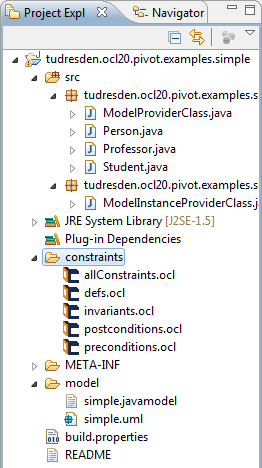
\includegraphics[width=0.6\linewidth]{figures/examples/simple02}
	\caption{The package explorer containing the project which is needed to run this tutorial.}
	\label{pic:example:simple02}
\end{figure}

The project provides a model file which contains the simple class diagram (the model file is located at \model{model/simple.uml}) and the constraint file we want to interpret (located at \model{constraints/\linebreak[0]allConstraints.ocl}). Listing \ref{lst:interpret:allConstraints} shows the constraints defined in the constraint file.

\lstset{
  language=OCL
}
\begin{lstlisting}[caption={The constraints contained in the constraint file.}, captionpos=b, label=lst:interpret:allConstraints, float]
-- The age of Person can not be negative.
context Person
inv: age >= 0

-- Students should be 16 or older.
context Student
inv: age > 16

-- Proffesors should be at least 30.
context Professor
inv: not (age < 30)

-- Returns the age of a Person.
context Person
def: getAge(): Integer = age

-- Before returning the age, the age must be defined.
context Person::getAge()
pre: not age.oclIsUndefined()

-- The result of getAge must equal to the age of a Person.
context Person::getAge()
post: result = age
\end{lstlisting}

First, the constraint file defines three simple invariants that denote, that the \model{age} of every \model{Person} must always zero or greater than zero. Furthermore, the \model{age} of every \model{Student} must be greater than 16 and the  \model{age} of every \model{Professor} does not have to be lesser than 30.

In addition to that the constraint file contains a definition constraint that defines a new operation \model{getAge()} which returns the \model{age} of a \model{Person}. A precondition checks, that the \model{age} must be defined before it can be returned by the operation \model{getAge()}. And finally, a postcondition checks, whether or not the result of the operation \model{getAge()} is the same as the \model{age} of the \model{Person}.



\section{Preparation of the Interpretation}

To prepare the interpretation we have to import the model \model{model/simple.uml} for which we want to interpret constraints into the \eclipse{Model Browser}. We use the import wizard for domain-specific models of the toolkit to import the model. This procedure is explained in Section \ref{intro:loadModel}. Furthermore, we have to import a model instance for which the constraints shall be interpreted into the \eclipse{Model Instance Browser}. We use another import wizard to import the model instance \model{bin/tudresden/ocl20/pivot/examples/simple\linebreak[0]/\linebreak[0]ModelProviderClass.class}. Finally, we have to import the constraint file \model{constraints/allConstraints.ocl} containing the constraints we want to interpret. The import is done by an import wizard again. Afterwards, the \eclipse{Model Browser} should look like illustrated in Figure \ref{pic:interpret:prepare01} and the \eclipse{Model Instance Browser} should look like shown in Figure \ref{pic:interpret:prepare02}.

\begin{figure}[!htbp]
	\centering
	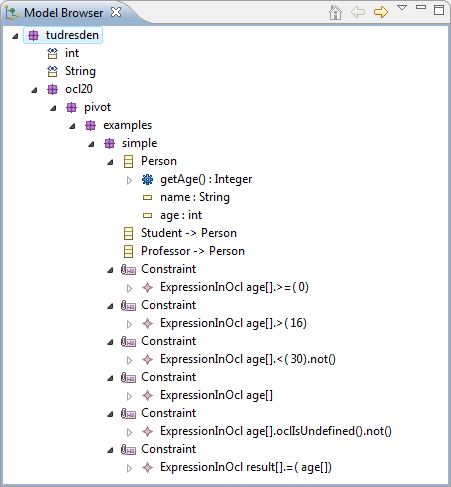
\includegraphics[width=0.8\linewidth]{figures/interpreter/prepare01}
	\caption{The model browser containing the simple model and its constraints.}
	\label{pic:interpret:prepare01}
\end{figure}

\begin{figure}[!htbp]
	\centering
	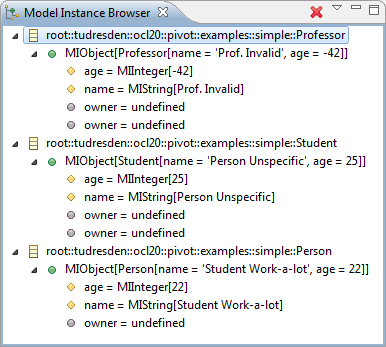
\includegraphics[width=0.7\linewidth]{figures/interpreter/prepare02}
	\caption{The model instance browser containing the simple model instance.}
	\label{pic:interpret:prepare02}
\end{figure}

The loaded model instance contains three instances of the classes defined in the Simple Example model. One instance of \model{Person}, one instance of \model{Student} and one instance of \model{Professor}. For these three instances we now want to interpret the imported constraints.



\section{OCL Interpretation}

Now we can start the interpretation. To open the \acs{OCL}2 Interpreter we use the menu option \reference{Dresden OCL2 > Open OCL2 Interpreter}. The \eclipse{OCL2 Interpreter View} should now be visible (see Figure \ref{pic:interpret:interpret01}).

\begin{figure}[!htbp]
	\centering
	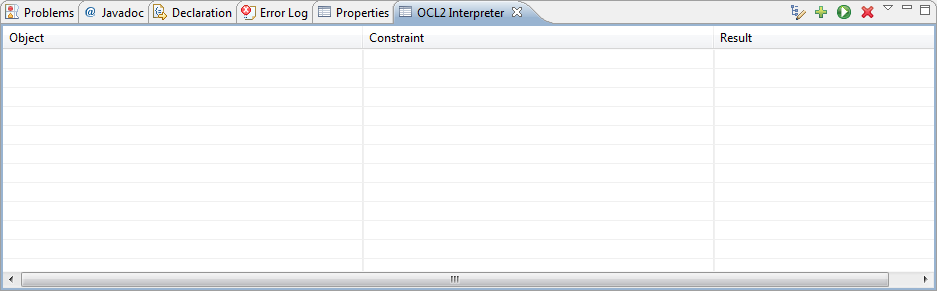
\includegraphics[width=1.0\linewidth]{figures/interpreter/interpret01}
	\caption{The OCL2 Interpreter containing no results.}
	\label{pic:interpret:interpret01}
\end{figure}

By now, the \eclipse{OCL2 Interpreter View} does not contain any result. Besides the results table, the view provides four buttons to control the \acs{OCL}2 Interpreter. The buttons are shown in Figure \ref{pic:interpret:interpret02}. With the first button (from left to right) constraints can be prepared for interpretation. The second button can be used to add variables to the \keyword{Interpreter Environment}. The third button provides the core functionality, it can be used to start the interpretation. And finally, the fourth button provides the possibility to delete all results from the \eclipse{OCL2 Interpreter View}. The functionality of the buttons will be explained below.

\begin{figure}[!htbp]
	\centering
	
\includegraphics[width=0.5\linewidth]{figures/interpreter/interpret02}
	\caption{The buttons to control the OCL2 Interpreter.}
	\label{pic:interpret:interpret02}
\end{figure}


\subsection{Interpretation of Constraints}

To interpret constraints, we simple select them in the \eclipse{Model Browser} and press the button to interpret constraints (the third button from the left). First, we want to interpret the three invariants defining the range of the \model{age} of \model{Persons}, \model{Students} and \model{Professors}. We select them in the \eclipse{Model Browser} (see Figure \ref{pic:interpret:interpret03}) and click the \eclipse{Interpret} button. The result of the interpretation is now shown in the \eclipse{\acs{OCL}2 Interpreter View} (see Figure \ref{pic:interpret:interpret04}).

\begin{figure}[!htbp]
	\centering
	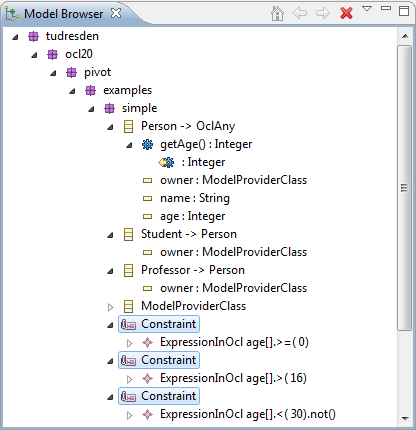
\includegraphics[width=0.7\linewidth]{figures/interpreter/interpret03}
	\caption{The three age invariants selected in the Model Browser.}
	\label{pic:interpret:interpret03}
\end{figure}

\begin{figure}[!htbp]
	\centering
	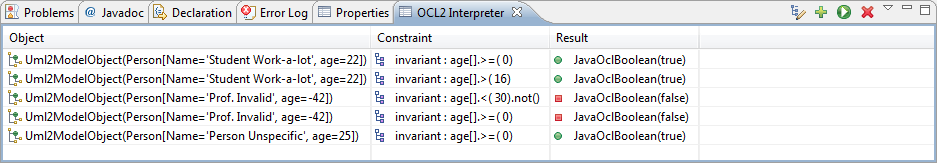
\includegraphics[width=1.0\linewidth]{figures/interpreter/interpret04}
	\caption{The results of the three age invariants for all model instances.}
	\label{pic:interpret:interpret04}
\end{figure}

The invariant \model{age >= 0} has been interpreted for all three model objects. The results for the \model{Person} and the \model{Student} instances are \model{true} because their \model{age} is greater than zero. The result for the \model{Professor} instance is \model{false} because its \model{age} is \model{-42}.

The two other invariants were only interpreted for the \model{Student} or the \model{Pro\-fessor} instance because their context was not the class \model{Person} but the class \model{Student} or the class \model{Professor}. Again the \model{Student's} result is \model{true} and the \model{Professor's} result is \model{false}.


\subsection{Preparation of Constraints}

Some constraints cannot be interpreted because they are no constraints in the natural sense of the word constraint. \acs{OCL} enables us to use constraints to define new attributes and methods or to initialize attributes and methods. Such \model{def}, \model{init} and \model{body} constraints cannot be interpreted because they have no result. They can only be used to alter the results of other constraints which shall be interpreted.

The Simple Example constraint file contains a definition constraint, which defines the method \model{getAge()} for the class \model{Person}. Before we can refer to this method in other constraints we have to prepare the definition constraint to ensure, that the interpretation of other constraints will finish with the right results.

To prepare the definition constraint, we select it in the \eclipse{Model Browser} (see Figure \ref{pic:interpret:interpret05}) and click the \eclipse{Prepare} button (the first button from the left).

\begin{figure}[!htbp]
	\centering
	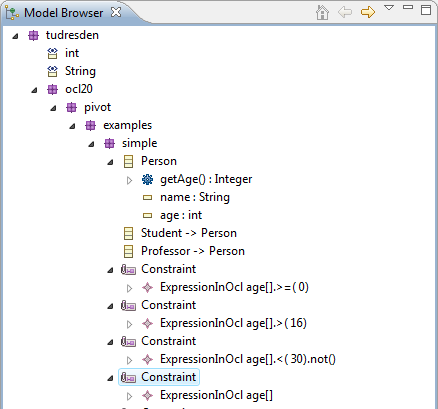
\includegraphics[width=0.7\linewidth]{figures/interpreter/interpret05}
	\caption{The definition constraint selected in the Model Browser.}
	\label{pic:interpret:interpret05}
\end{figure}

The preparation does not result with a visible result in the \eclipse{OCL2 Interpreter View}. But the method definition of the constraint has been added to the \keyword{Interpreter Environment} of the \acs{OCL}2 Interpreter. Thus, we can interpret the next constraint now. This constraint is the precondition which checks that the \model{age} of any \model{Person} must be defined before the method \model{getAge()} can be invoked.

We select the constraint in the \eclipse{Model Browser} (see Figure \ref{pic:interpret:interpret06}) and click the \eclipse{Interpret} button. The result of the interpretation is shown in figure \ref{pic:interpret:interpret07}.

\begin{figure}[!htbp]
	\centering
	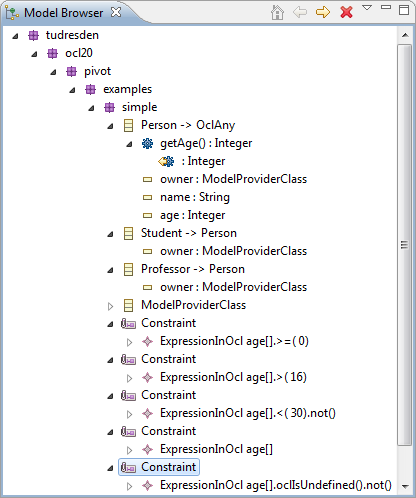
\includegraphics[width=0.7\linewidth]{figures/interpreter/interpret06}
	\caption{The precondition selected in the Model Browser.}
	\label{pic:interpret:interpret06}
\end{figure}

\begin{figure}[!htbp]
	\centering
	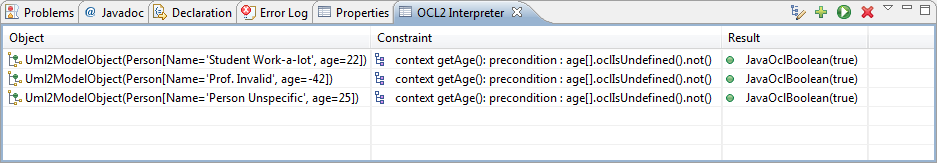
\includegraphics[width=1.0\linewidth]{figures/interpreter/interpret07}
	\caption{The results of the precondition for all model instances.}
	\label{pic:interpret:interpret07}
\end{figure}

The interpretation finishes for all three instances successfully because the attribute \model{age} has been set for all three instances.


\subsection{Adding Variables to the Environment}

By preparing the definition constraint we added some information to the \keyword{Interpretation Environment} that was necessary to interpret other constraints. For some constraints we have to add further information which can not be provided by the preparation of other constraints.

For example, our last constraint a postcondition compares the result of the method \model{getAge()} with the attribute \model{age} of the referenced \model{Person} instance. Therefore, \acs{OCL} provides the special variable \model{result} in postconditions which contains the result of the constrained method's execution. Using the \eclipse{\acs{OCL}2 Interpreter View} we cannot execute the method \model{getAge()} and store the result in the \model{result} variable. We can interpret the postcondition in a specific context which has to be prepared by hand only. We have to set the result variable manually.

If we interpret the postcondition constraint (the sixth and last constraint in the \eclipse{Model Browser}) without setting the \model{result} variable, the constraint results in a \model{undefined} result for all three model instances (see Figure \ref{pic:interpret:interpret08}).

\begin{figure}[!htbp]
	\centering
	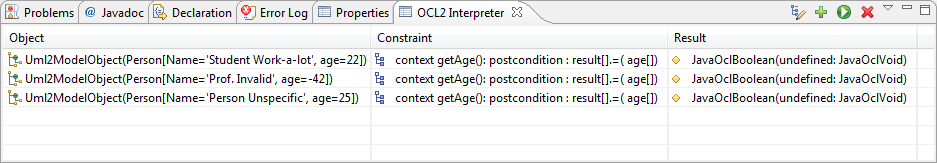
\includegraphics[width=1.0\linewidth]{figures/interpreter/interpret08}
	\caption{The results of the postcondition without preparing the result variable.}
	\label{pic:interpret:interpret08}
\end{figure}

To prepare the variable we click on the button to add new variables to the Interpreter Environment (the second button from the left) and a new window opens which we can use to specify new variables. We enter the name \model{result}, select the variable type \model{Integer} and enter the value \model{25}. Then we press the \eclipse{OK} button (see Figure ref{pic:interpret:interpret09}. The result variable has now been added to the Interpreter Environment.

\begin{figure}[!htbp]
	\centering
	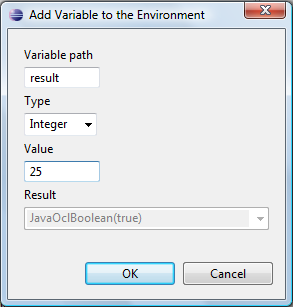
\includegraphics[width=0.5\linewidth]{figures/interpreter/interpret09}
	\caption{The window to add new variables to the environment.}
	\label{pic:interpret:interpret09}
\end{figure}

\begin{figure}[!htbp]
	\centering
	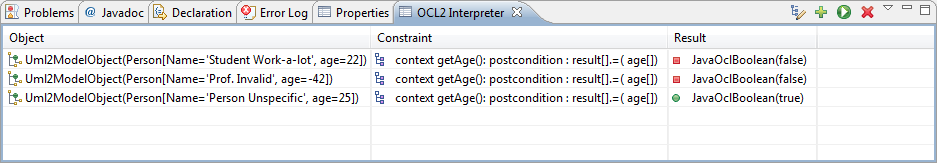
\includegraphics[width=1.0\linewidth]{figures/interpreter/interpret10}
	\caption{The results of the postcondition with result variable preparation.}
	\label{pic:interpret:interpret10}
\end{figure}

Now we can interpret the postcondition again. The result is shown in Figure \ref{pic:interpret:interpret10}. The results for the \model{Student} and \model{Professor} instances are both \model{false} because their \model{age} attribute is not equal to \model{25} and thus the \model{result} value does not match to the \model{age} attribute. But the interpretation for the \model{Person} instances succeeds because its age is \model{25}.




\section{Summary}
  
This Chapter described how \acs{OCL} constraints can be interpreted using the \acs{OCL}2 Interpreter of \acl{DOT4Eclipse}. The preparation and interpretation of constraints has been explained, the addition of new variables to the Interpreter Environment has been shown.